% p29-ext-f-completes-the-following-diagram.tex
%
% Source:   Carl A. Gunter and Dana S. Scott, "Semantic Domains".
%           ScottDomains/papers/Gunter Scott 1990.pdf
% Physical page: 29          Printed page: 28
% Section:  5.3 Universal and closure properties.
% Unnamed in the paper (no figure number). Introduced by Theorem 12:
%   "Theorem 12  Let D be a domain. Suppose <E, *> is a continuous algebra
%    which satisfies T-natural. For any continuous f : D -> E, there is a
%    unique homomorphism ext(f) : D-natural -> E which completes the following
%    diagram:"
%
% Content: D-natural is the free continuous algebra (the convex powerdomain)
% over D; the singleton map {|.|} : D -> D-natural is the unit. Same triangle
% shape as the smash and lift diagrams. Vertices 3, arrows 3 (2 solid,
% 1 dashed).
%
% Geometry measured from a 300 dpi render of the region and divided by
% 118.11 px/cm.
%
\documentclass[border=6pt]{standalone}
\usepackage{tikz}
% the paper's singleton bracket {|.|}; the negative kerns must stay small
% enough that the vertical bars are not swallowed by the braces
\newcommand{\sglt}{\{\mkern-3.5mu|\mkern1mu\cdot\mkern1mu|\mkern-3.5mu\}}
\begin{document}
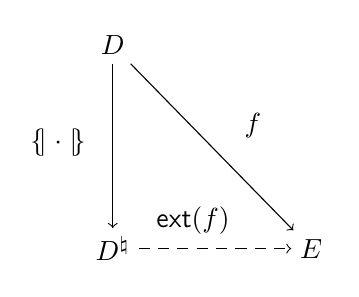
\begin{tikzpicture}[
  x=1cm, y=1cm,
  every node/.style={inner sep=1pt},
  open/.style={circle, draw, fill=white, minimum size=4pt, inner sep=0pt},
  solid/.style={circle, draw, fill=black, minimum size=5pt, inner sep=0pt},
  edge/.style={draw, line width=0.4pt},
  % added for the commutative diagrams: object nodes, and the paper's two
  % arrow kinds -- solid for a named map, dashed for the unique completing map
  obj/.style={inner sep=3pt},
  arrow/.style={draw, line width=0.4pt, ->},
  darrow/.style={draw, line width=0.4pt, ->, dash pattern=on 4pt off 3pt}]

  % vertices
  \node[obj] (d)   at (0.00,2.58) {$D$};
  \node[obj] (dna) at (0.00,0.00) {$D^{\natural}$};
  \node[obj] (e)   at (2.52,0.00) {$E$};

  % arrows
  \draw[arrow]  (d)   -- (dna);
  \draw[arrow]  (d)   -- (e);
  \draw[darrow] (dna) -- (e);

  % labels printed inside the picture
  \node[anchor=east] at (-0.30,1.34) {$\sglt$};
  \node at (1.78,1.56) {$f$};
  \node[anchor=south] at (1.02,0.14) {\textsf{ext}$(f)$};
\end{tikzpicture}
\end{document}
